\chapter{LibGen -{} Library Generator -{} Parts 2 \& 3}

\section{Introduction}
\label{ch32-intro}%\hyperlabel{ch32-intro}%

\begin{note}
This chapter was originally submitted as one article. Due to space
      restrictions in QL Today, Geoff and Jochen had to split it into two.
      They appeared in Volume 17 issues 1 and 2. Hence the somewhat strange title here!

The corrections posted in the next chapter have been applied to
      this one. Obviously, I couldn't get Jochen to reprint all the affected
      QL Today magazines, so I have been able to correct them here. You know
      what I mean!
\end{note}

\section{LibGen Processing}
\label{ch32-lib-gen-processing}%\hyperlabel{ch32-lib-gen-processing}%

The code for LibGen\program{LibGen}  \emph{should} work as follows:
\begin{enumerate}
\item{The program starts with only the `Esc', `Move' and `Sym file'
        loose items enabled. Everything else is unavailable.
}
\item{The user hits `Sym file'. This causes all loose items except
        `Move' and `Esc' are set to unavailable -{} in case the edit is aborted,
        or an error occurs. The user then types in the name of the sym\_lst
        file created by George's sym\_bin utility.
        The user then terminates or aborts the edit.

On a successful edit, the affected loose items are made
        available again (except `Save'). On an aborted edit, or error, the
        loose items are left unavailable, except for `Sym file' which is reset
        to available. The user will remain at this step until a successful
        edit completes.
}
\item{The `Sym file' name entered by the user is changed by removing
        the `\_sym\_lst' extension and adding `\_lib' in its place to form the
        `Lib file' default file name, and by having the extension `\_bin' added
        on to form the `Bin file' default value. These defaults are displayed
        in the appropriate information windows.
}
\item{When a suitable symbol file name has been entered, all the
        application specific loose items will be enabled with the exception of
        `Save'. The user may use the `Lib file' and `Bin file' loose items to
        amend the default file names for the two files that will be created by
 LibGen on hitting `Save'.
}
\item{When the user hits the `Load', the `Sym file' is opened and read
        in two passes. The first counts the number of \emph{code offset
 }lines that will be added to the menu. The second pass will
        add each one to the buffer allocated, dynamically, for this purpose.
        At end of file, the file will be closed and the buffer added to the
        application sub-{}window as a menu, All items in the menu will be
 \emph{selected} by default. If the file loads correctly,
        the `Save' loose item will be enabled.
}
\item{When the user hits `Save', the currently selected items in the
        application sub-{}window menu will be written out to the `Lib file',
        followed by a command to import the `Bin file'. When complete, the
        file will be closed and all items will be set to the starting position
        where only `Sym file' is available.
}
\end{enumerate}

\section{LibGen Code}

The first version of the code does nothing more than display the
    window on the screen and enter the loop to read the pointer and, as usual,
    this will only return (from WMAN) when an event
    happens or an error occurs in either a loose item hit routine or the
    application menu hit routine. The following code is pretty much a template
    for any
 SETW/EasyPEasy built
    applications. It displays the window on screen and that's about all it
    does -{} pressing the ESC key or HITting/DOing the `Esc' loose item will end
    the program.

\begin{lstlisting}[firstnumber=1,]
         bra   start
         dc.w  0
         dc.w  $4afb

fname    dc.w  fname_e-fname-2
         dc.b  "LibGen - Library Generator"
fname_e  ds.b  0
         ds.w  0

;---------------------------------------------------------------------
; We need the various equates files etc.
;---------------------------------------------------------------------
         in win1_georgegwilt_peass_keys_pe
         in win1_georgegwilt_peass_qdos_pt
         in win1_georgegwilt_peass_keys_wwork
         in win1_georgegwilt_peass_keys_wstatus
         in win1_georgegwilt_peass_keys_wman
         in win1_georgegwilt_peass_keys_wdef

;---------------------------------------------------------------------
; Offsets into the data area for working storage.
;---------------------------------------------------------------------
id       equ 0                   Channel id storage.
wmvec    equ 4                   WMAN vector storage.
slimit   equ 8                   IOP_FLIM output buffer.
\end{lstlisting}

Departing from the template next, I define meaningful names for my
    loose items and information windows. It's much easier to determine which
    loose item or information window is being affected when reading the code
    back in 6 months or so, when you read names as opposed to a list of
    numbers.

I could have simply used an `IN' directive and a separate file at
    this point, which may prove useful for larger applications, but for now,
    I'm simply including the equates directly into my template. You will note
    that the three strings I'm defining storage for are initialised to be zero
    length.

This is important because when we come to allow the user enter the
    symbol filename, the existing string is presented for editing. If we left
    the data uninitialised, we could get some interesting results as random
    strings were presented for editing. It's much better to initialise to an
    empty string as part of the program initialisation.

\begin{lstlisting}[firstnumber=1,]
;---------------------------------------------------------------------
; Loose items we may need.
;---------------------------------------------------------------------
li_symfile equ 2
li_libfile equ 3
li_load    equ 4
li_save    equ 5
li_binfile equ 6

;---------------------------------------------------------------------
; Information windows we may need.
;---------------------------------------------------------------------
iw_symfile equ 2
iw_libfile equ 3
iw_binfile equ 5

;---------------------------------------------------------------------
; Working buffer for the three file names. 40 characters allowed. The
; three strings are initialised to be of zero length.
;---------------------------------------------------------------------

sym_buffer dc.w 0                A zero word count is useful!
           ds.w 20               Space for 40 characters inc N/L.

lib_buffer dc.w 0
           ds.w 20

bin_buffer dc.w 0
           ds.w 20

;---------------------------------------------------------------------
; Buffer for the 2 extra filename extensions we desire. These will be
; added to the end of the supplied sym file name from the user.
;---------------------------------------------------------------------
lib_extn dc.w lib_extn_e-lib_extn-2
         dc.b '_lib'
lib_extn_e equ *

bin_extn dc.w bin_extn_e-bin_extn-2
         dc.b '_bin'
bin_extn_e equ *
\end{lstlisting}

The remainder of the code is back to the template again.

\begin{lstlisting}[firstnumber=1,]
;---------------------------------------------------------------------
; Console definition, and code to open it.
;---------------------------------------------------------------------
con      dc.w con_e-con-2        Size of channel definition.
         dc.b 'con_'
con_e    equ *

op_con   lea  con,a0             We want a console.
         moveq #-1,d1            For this job.
         moveq #0,d3             Timeout.
         moveq #io_open,d0
         trap #2                 Do it.
         rts

;---------------------------------------------------------------------
; The main code itself.
;---------------------------------------------------------------------
start    lea (a6,a4.l),a6        Make A6 point to the job's dataspace.
         bsr op_con              Open a con channel.
         move.l a0,id(a6)        And store the channel id.
         moveq #iop_pinf,d0      Trap to get Pointer Information.
         moveq #-1,d3            Timeout.
         trap #3                 Do it.
         tst.l d0                Is ptr_gen present?
         bne sui                 No, bale out via SUI.
         move.l a1,wmvec(a6)     Yes, store the WMAN vector.
         beq sui                 Oops! WMAN wasn't actually found.

flim     movea.l a1,a2           The WMAN vector is required in A2.
;                                The channel id is already in A0.
         lea slimit(a6),a1       Result buffer.
         moveq #iop_flim,d0      Query maximum size of window.
         moveq #0,d2             D2 is required to be zero.
;                                D3 is the timeout.
         trap #3                 Do it.
         tst.l d0                Did it work?
         bne sui                 No, exit via SUI.

         subi.l #$C0008,(a1)     Minus 12 (width) & 8 (height).
         lea wd0,a3              Get address of window definition.
         move.l #ww0_0,d1        Get size of the working definition.
         bsr getsp               Easy PEasy - ALCHP memory and set A0.
         movea.l a0,a4           Which we save in A4.
         lea wst0,a1             Status area address.
         movea.l a1,a0           Copy to A0.
         moveq #wst0_e-wst0-1,d1 How many bytes to clear - 1.


\end{lstlisting}

So far, we have seen most of this before. However, we depart from
    the normal template in the next few lines, from label
 \texttt{st\_clr} onwards.

\begin{lstlisting}[firstnumber=1,]
st_clr   clr.b (a0)+             Clear one byte.
         dbf d1,st_clr           Then the remainder.

st_loose lea ws_litem+li_libfile(a1),a0  Status byte for Lib file.
         moveq #3,d1             Four status bytes to reset.

st_unav  move.b #wsi_unav,(a0)+  Set loose item to unavailable.
         dbf d1,st_unav          And the rest.
\end{lstlisting}

First we initialise all of the status area, including the loose
    items, to a byte of zero, in the normal manner with the small loop at
 \texttt{st\_clr}. For the loose items, this happens to be the
    status code for available. However, as we don't want every loose item to
    be available when the program starts, the code at
 \texttt{st\_loose} onwards will set the status byte for the 4
    loose items in question, to unavailable -{} there is another way I can set
    these 4 status bytes, as we shall see later on in the code. These will be
    made available by the code in other loose item hit routines as
    appropriate.

I can use a loop at \texttt{st\_unav} because of the
    order I created my loose items in SETW. The 4
    loose items, `Lib file', `Load', `Save' and `Bin file' are set to
    unavailable in this loop. If you created your loose items in a different
    order, you may need to do each one individually.

Because of this status byte being set in the application's
    initialisation, these four loose items will be unavailable when the
    application displays its window on screen.

Back to the template code again.

\begin{lstlisting}[firstnumber=1,]
         movea.l id(a6),a0       Channel ID in A0.
;                                A1 = status area.
;                                A3 = window definition.
;                                A4 = working definition.
         move.l wd_xmin+wd_rbase(a3),d1  Get minimum size.
         andi.l #$FFF0FFF,d1     Mask off scaling factors.
         jsr wm_setup(a2)        Set up the window.

         moveq #-1,d1            Use the current pointer position.
         jsr wm_prpos(a2)        Position as a primary window, then.
         jsr wm_wdraw(a2)        Draw the contents.

;---------------------------------------------------------------------
; The main Read Pointer loop.
;---------------------------------------------------------------------
wrpt     jsr wm_rptr(a2)         Enter read pointer loop in WMAN.
         beq.s no_err            Since D0 is zero D4 is non zero.
         bra sui                 An error occurred exit via SUI.

no_err   movea.l (a4),a1         Status area address.
         btst #pt__can,wsp_weve(a1) Check for CANCEL event.
         bne sui                 Exit.

         bra.s wrpt              No more events, read pointer again.
\end{lstlisting}

I have only included a check for the CANCEL event in the above code.
    Normally there would be SLEEP and SIZE event checking, probably as an
    absolute minimum. However, I need to keep the code size to a minimum for
    the magazine, so these applications will only have the minimum
    required.

Next comes the loose items and application window hit routines. In
    this first version of the code, the loose item hit routines for the
    following 4 loose items simply do nothing except reset the status from
    selected back to available when hit.

\begin{lstlisting}[firstnumber=1,]
;---------------------------------------------------------------------
; Dummy, for now, loose item action routines.
;---------------------------------------------------------------------
afun0_6  bra li_reset            Bin file.
afun0_5  bra li_reset            Save.
afun0_4  bra li_reset            Load.
afun0_3  bra li_reset            Lib file.
afun0_2  bra li_reset            Sym file.
\end{lstlisting}

Before we delve into proper hit routines, the \tablename~\ref{tab:LooseItemHitRoutineRegisters32} is a
    reminder of what registers are set on entry to a loose item hit
    routine.


\begin{table}[htbp]
\centering
\begin{tabular}{l p{0.8\textwidth}}
\toprule
\textbf{Register} &\textbf{Description}  \\
\midrule
%
D1.L & High word = pointer X position, Low Word = pointer Y position.\\
D2.W & Selection keystroke letter, in its upper cased format, or 1 = Hit/SPACE or 2 = DO/ENTER.\\ D2.W & may be an event code if an event triggered this action.\\
D4.B & An event number - if an event triggered this action routine.\\
A0.L & Channel id.\\
A1.L & Pointer to the status area.\\
A2.L & WMAN vector.\\
A3.L & Pointer to loose menu item.\\
A4.L & Pointer to window working definition.\\
%
\bottomrule
\end{tabular}
\caption{Loose Item Hit Routine Registers}
\label{tab:LooseItemHitRoutineRegisters32}
\end{table}

Next up is the first of our working loose item hit routines. This
    one handles the `Move' action. Also showing in the following code is the
    routine where we reset the appropriate loose item's status back to
    available from the currently selected status.

You can see from the above, that the majority of the loose items
    simple reset their status and exit back to
 WMAN.

\begin{lstlisting}[firstnumber=1,]
;---------------------------------------------------------------------
; MOVE hit. Move the window.
;---------------------------------------------------------------------
afun0_1  bsr move


;---------------------------------------------------------------------
; Reset current loose item status to available & redraw. Entry point
; li_reset resets the current loose item while entry at li_rest must
; have a loose item number in D1.W.
;---------------------------------------------------------------------
li_reset move.w wwl_item(a3),d1  Get the loose item number.

li_rest  move.b #wsi_mkav,ws_litem(a1,d1.w) Set status to available.
         moveq #-1,d3            Request selective redraw.
         jsr wm_ldraw(a2)        Do it.
         bra.s li_done
\end{lstlisting}

There are two entry points here, the first at
 \texttt{li\_reset} handles the current loose item. If entry is
    at \texttt{li\_rest} then D1.W should be holding the
    appropriate loose item number.

Within a hit routine, as you may remember, A1 holds the pointer to
    the status area and A3 points at the definition of the loose item within
    the \emph{working definition}. By extracting the loose item
    number from the definition and adding it to A1 plus the offset to the
    start of the status bytes for the loose items, we can change the status to
 \texttt{wsi\_mkav} which is actually the value available +
    redraw.

The code then calls \texttt{wm\_ldraw} to redraw only
    those loose items which have the redraw bit set. This avoids flicker and
    doing unnecessary work redrawing unchanged loose items. When redrawn, the
    redraw bit is cleared by WMAN, leaving the
    status at available.

The code finishes by exiting through \texttt{li\_done} to
    clear out the D0 and D4 registers to indicate no errors and no events.
    After this, it returns back to WMAN and back
    into the pointer loop.

\begin{lstlisting}[firstnumber=1,]
;---------------------------------------------------------------------
; ESC pressed, set cancel event and exit.
;---------------------------------------------------------------------
afun0_0  bset  #pt__can,wsp_weve(a1) Set the CANCEL event bit.
         moveq #pt__can,d4       CANCEL event number in D4.
         bra.s li_exit


li_done  moveq #0,d4             No events.

li_exit  moveq #0,d0             No errors.
         rts                     Exit, and exit from wm_rptr too.



;---------------------------------------------------------------------
; Application sub-window hit routine
;---------------------------------------------------------------------
ahit0    moveq #0,d4             No events.
         moveq #0,d0             No errors.
         rts                     Exit back to the read pointer loop.
\end{lstlisting}

The code that handles a hit on the `Esc' loose item shows the
    alternative manner of handling loose items. It simply sets the CANCEL
    event bit in the event register in the status area (addressed by A1), sets
    the event code in D4 and exits back to WMAN     with D0 set to show no errors.

Having an event code in D4 causes WMAN to
    exit from the pointer reading loop and returns back to
 WMAN with D4 set.
 WMAN will see that an event has been set in D4
    and this will cause a return to our own application code at label
 \texttt{no\_err} (a long way above!). The code there checks for
    the CANCEL event and, if found, exits the program.

\begin{note}
You may be wondering why we gave the ESC loose item a keystroke
      appropriate to the CANCEL event number (3) when we did a little editing
      of the file created by SETW in the last
      article, and why we have to have a loose item hit routine that sets the
      CANCEL event? Surely WMAN handles all
      that?

Well, if you comment out the first two instructions at
 \texttt{afun0\_0} above, reassemble and execute the program
      and then HIT or DO the ESC loose item, you will see it become selected,
      but the program still runs.

However, if you press ESC, WMAN handles
      that and exits from the program. So, we must have the hit routine cause
      the program to exit when the loose item is HIT or DOne because
 WMAN isn't seeing the ESC key being pressed
      to cause an exit. The hit routine for the lose item sets the CANCEL
      event which causes the return to WMAN to
      return to our code and thus, exits from the program. Simple?

Even if there was no loose item to explicitly close the program,
      as long as the application checked for a CANCEL event, as
 LibGen does, we can still close the program
      by pressing the ESC key because WMAN       intercepts the ESC key, generates the CANCEL event and exits back to our
      application code where, hopefully, events are checked for.
\end{note}

Immediately following the `Esc' loose item code we have a dummy
    `does nothing yet' routine for the application window hit routine.

Finally, the last few lines pull in the window definition created by
 SETW and George's
 EasyPEasy library.

\begin{lstlisting}[firstnumber=1,]
;---------------------------------------------------------------------
; Pull in our window definition file.
;---------------------------------------------------------------------

         in  win1_source_qltoday_libgenWin_asm

;---------------------------------------------------------------------
; We need George's Easy PEasy code next.
;---------------------------------------------------------------------

         in  win1_georgegwilt_peass_peas_sym_lst
         lib win1_georgegwilt_peass_peas_bin

;---------------------------------------------------------------------
; And finally, George's sprites.
;---------------------------------------------------------------------

         in  win1_georgegwilt_peass_csprc_sym_lst
         lib win1_georgegwilt_peass_csprc_bin
\end{lstlisting}

If you save and assemble the above, you should be able to execute
    the utility and see it in action. You will only have the `Sym file'
    action, other than move or `Esc' available to you on startup and all the
    filenames will be blank.

At the moment though, even if the `Sym file' loose item is enabled,
    the hit routine does nothing other than set the status back to
    available.

Now that we have the main part of the code to handle the
    initialisation, display and so on working, it's time to add some meat to
    the bones of what we have.

\section{Handling the Sym File Loose Item}
\label{ch32-handling-sym-file}%\hyperlabel{ch32-handling-sym-file}%

Looking back at our LibGen processing
    description above, we have already completed the first step. Step 2
    requires us to let the user type in the symbol file name when the `Sym
    file' loose item is HIT or DOne. Additionally, the `Load' loose item
    becomes available when the action routine completes.

Keeping it simple for now, type in the following code at the
    location of the label \texttt{afun0\_2} which is currently
    showing a branch to the \texttt{li\_reset} routine. The
    following code replaces that which currently exists.

\begin{lstlisting}[firstnumber=1,]
;---------------------------------------------------------------------
; SYM FILE loose item action routine.
;---------------------------------------------------------------------
afun0_2  movem.l d5-d7/a0-a4,-(a7) Preserve important registers.
         bsr sym_hit               Do it all.
         movem.l (a7)+,d5-d7/a0-a4 Restore important registers.
         moveq #li_load,d1       Load loose item.
         bsr li_rest             Make Load available.
         bra li_reset            Make Sym file available.

sym_hit  rts                     Temporary code for now.
\end{lstlisting}

Once again, assemble and execute the code. Now when you HIT or DO
    the `Sym file' loose item, you should see the `Load' loose item become
    available.

The code preserves the registers we need to preserve over an action
    routine, branches out to our temporary hit code and on return, restores
    the registers before setting the `Load' loose item's status byte to
    available. Finally, the code exits via the \texttt{li\_reset}     
    routine which causes the current loose item (`Sym file') to be reset to
    available and redrawn.

That's the easy bit done. The next part gets into the real code for
    a HIT or DO on the `Sym file' loose item. Replace the current one line at
    label \texttt{sym\_hit} with the following code.

\begin{lstlisting}[firstnumber=1,]
;---------------------------------------------------------------------
; This code carries out all the nasty work for a hit on the Sym file
; loose item. It is called from afun0_2 above.
;---------------------------------------------------------------------
sym_hit  moveq #iw_symfile,d1    Info window number in d1.w.
         lea sym_buffer,a3       Current sym file buffer.
         moveq #1,d2             Blue Ink colour.
         bsr iw_input            Get input from desired info window.
         blt.s sh_exit           Something went wrong, bale out.
\end{lstlisting}

It's at this point that having some equates defined for the various
    information windows comes in handy. The code above starts off by loading
    D1 with the number of the information window that will eventually allow us
    to type in the file name and which will also display the file name when we
    have typed it.

A3 holds the address of a buffer, which we set up way back at the
    start. On the first run of the program, this buffer holds a zero length
    string. After it has been run and used, whatever the last symbol file name
    that you typed in will be there.

D2 needs to hold the ink colour, blue in this case, as we will be
    clearing the information window shortly. The code is written so that when
    any information window is being used to edit data, the ink colour is blue,
    but when the data has been entered, it is printed with black ink.

We then branch off to a subroutine names
 \texttt{iw\_input} to allow the user the ability to type in a
    file name directly into the appropriate information window. This routine
    will be discussed later.

On return, if any errors were detected, we bale out. The calling
    code can handle this, as desired. In this example,
 LibGen does nothing with errors. The program
    continues to run, in this case, and you can try again, if desired.

\begin{lstlisting}[firstnumber=1,]
;---------------------------------------------------------------------
; Did we abort the edit?
;---------------------------------------------------------------------
sh_esc   cmpi.w #27,d1           ESC?
         beq.s sh_sym            Yes.
\end{lstlisting}

The \texttt{iw\_input} routine sets the terminating
    character in D1. This can be ESC, ENTER or the Up or Down Arrows. We are
    interested only in the ESC key as this implies that the user decided to
    abort the edit.

If we find the ESC key terminated the edit, we bale out via the
 \texttt{sh\_sym} label, which tidies up the potential garbage
    that is now showing in the information window. The code at
 \texttt{sh\_sym} also prints the file name in black ink as
    opposed to the editing colour of blue.

If the user terminated the edit normally, we have completed step 2
    in our LibGen processing and are ready to carry
    out step 3. The following code does exactly that.

\begin{lstlisting}[firstnumber=1,]
;---------------------------------------------------------------------
; Copy sym filename to other buffers and add appropriate extensions.
; The sym file is assumed to have a '_sym_lst' extension present.
;---------------------------------------------------------------------
sh_ok    move.l a2,-(a7)         Preserve WMAN vector.

         lea lib_buffer,a2       Destination buffer.
         lea sym_buffer,a3       Source buffer.
         bsr cp_string           Copy to lib file.
         subi.w #8,(a2)          Strip off '_sym_lst'.
         bcs.s sh_err            Negative is bad!
         lea lib_extn,a3         Lib file extension.
         bsr ap_string           Add lib file extension.

         lea bin_buffer,a2       Destination buffer.
         lea sym_buffer,a3       Source buffer.
         bsr cp_string           Copy to bin file.
         subi.w #8,(a2)          Strip off '_sym_lst'.
         bcs.s sh_err            Negative is bad!
         lea bin_extn,a3         Bin file extension.
         bsr ap_string           Add it to the bin file.

         moveq #0,d2             Black ink required for filenames.
         move.l (a7)+,a2         Restore WMAN vector.
         moveq #iw_libfile,d1    Info window required.
         lea lib_buffer,a3       String address.
         bsr iw_print            Print lib file.

         moveq #iw_binfile,d1    Info window.
         lea bin_buffer,a3       String address.
         bsr iw_print            Print bin file.
         bra.s sh_sym            Skip error handling.

;---------------------------------------------------------------------
; If the lib or bin filename lengths go negative after subtracting the
; 8 bytes necessary for the assumed '_sym_lst' extension, we bale out
; but need to tidy the stack first.
;---------------------------------------------------------------------
sh_err   move.l (a7)+,a2         Get the WMAN vector again.

\end{lstlisting}

The code above simply copies the file name entered by the user from
    the input buffer to the buffers set aside for the `Lib file' and `Bin
    file'. For each of these, the `\_sym\_lst' extension is removed and a new
    extension appropriate to the file name being generated is appended.

\begin{note}
You will note that there is not much in the way of error trapping
      going on here. This is, again, to keep code to a minimum. A proper
      application would do various checks to ensure that the symbol file
      actually existed, that it had the correct extension and so on, before
      manipulating the file name to create the defaults for the other two file
      names.

The only error trapping that is happening is a check that when
      subtracting 8 from the string length -{} to remove the characters
      `\_sym\_lst' -{} that the string length doesn't go negative. If it does, we
      bale out via \texttt{sh\_err} and \texttt{sh\_sym}       where we tidy up the display again.
\end{note}

The strings are moved around and appended to using some more useful
    routines in one of my libraries. These will be discussed later.

Finally, for this action routine, we have the following code which
    calls yet another of my library routines, \texttt{iw\_print},
    to clear the information window in question, and print the contents of the
    correct buffer to it.

\begin{lstlisting}[firstnumber=1,]
;---------------------------------------------------------------------
; Print the sym file name. We do this at the end of a normal edit and
; when the user aborts with ESC. This keeps the info window tidy.
;---------------------------------------------------------------------
sh_sym   move.w d1,-(a7)         Preserve the terminator keypress
         moveq #iw_symfile,d1    Information window desired.
         moveq #0,d2             Black ink.
         lea sym_buffer,a3       Filename to print.
         bsr iw_print            Print it.
         move.w (a7)+,d1         Restore the termintor keypress

sh_exit  rts
\end{lstlisting}

Unfortunately, at this point, if you assemble the code, you will see
    8 errors. All caused by a lack of my own library routines. The next
    section holds the code for the routines we are using, but have not yet
    created.

\section{The Utilities Library}
\label{ch32-utilities-library}%\hyperlabel{ch32-utilities-library}%

Scroll to the end of the file and add the following lines,
    obviously, you will adjust the file name to suit your own installation.
    Unless, of course, your setup is exactly the same as mine.

You may also note, that while I refer to the code as a library, it
    is not yet converted into one. When we complete
 LibGen, we shall use it to build a working
    library. (Does that count as recursion?)

\begin{lstlisting}[firstnumber=1,]
;---------------------------------------------------------------------
; And finally finally, my own utilities.
;---------------------------------------------------------------------

         in win1_source_qltoday_pe_utilities_asm
\end{lstlisting}

The code above goes just after the part where we pull in George's
    sprite code.

It is not possible for a reusable library's routines to make any
    assumptions about the use of registers outside of the library itself. To
    this end, each of the following routines will preserve any register that
    it uses, with the exception of registers that are documented to return a
    potentially useful value.

Create a new file with the name given above, in my case -{} yours may
    be different, and add the following routines to it.

The first subroutine is \texttt{IW\_INPUT} which allows
    an information window to be used to accept input from the user.

It works by calling the WMAN routine that
    sets the channel ID to the information window in question, then copies the
    current value of the string to be edited to a working buffer. A jump back
    into WMAN is made to allow the user to edit the
    string. The edit may be terminated by ENTER, ESC, Up arrow or Down
    arrow.

\begin{note}
The QPTR documentation states that the \emph{Condition
      Codes}, not D0, will be zero if ENTER was pressed, negative
      for any errors, and positive if ESC, Up or Down were used to terminate
      the edit. D0 will \emph{always} be zero at the end of an
      edit, unless any errors occurred whereupon, it will be negative.

The library routine \texttt{iw\_input} sets D0 to a
      positive value -{} actually 1 -{} when ESC, Up or Down arrow terminates the
      edit.
\end{note}

\begin{lstlisting}[firstnumber=1,]
;=====================================================================
; This file contains useful utilities for a Pointer Environment
; application. It's just crying out to become a library! ;-)
;---------------------------------------------------------------------
; IW_INPUT  - Get input from a designated information window.
; IW_PRINT  - Print a string to a designated information window.
; CP_STRING - Copy a string between two locations.
; AP_STRING - Append one string to the end of another.
;=====================================================================


;=====================================================================
; IW_INPUT : accept input from an information window. The routine has
;            a working buffer of 1024 characters maximum which is
;            more than enough for any information window width.
;=====================================================================
; Entry Registers:
;
; D1.W Information window number.
; D2.L Ink colour, or negative ink colour. See WM_SWINF documentation.
; A2.L WMAN vector.
; A3.L Pointer to string.
; A4.L Pointer to work def.
;---------------------------------------------------------------------
; Exit Registers:
;
; D1.W Terminating character: Enter, Esc, Up arrow, Down arrow.
; D2.L Preserved.
; A1.L Buffer pointer.
; A2.L Preserved.
; A3.L Buffer pointer.
; A4.L Preserved.
;---------------------------------------------------------------------
; Errors:
;
; D0 = negative: Any I/O error. Old string at (A3) unaffected.
; D0 = zero:     Enter terminated the edit. Old string at (A3) updated.
; D0 = Positive: Up, Down or ESC terminated the edit. Old string at (A3)
;                updated, unless ESC pressed.
;=====================================================================
iw_input movem.l a2-a3,-(a7)     Save WMAN vector & source buffer.

iw_copy  lea iw_buffer,a2        Copy destination buffer.
         bsr cp_string           Copy to work buffer.
         move.l (a7),a2          Get WMAN vector.

         jsr wm_swinf(a2)        Set channel to info window.
         bne.s iw_exit           Bale out on error.

         lea iw_buffer,a1        Edit buffer required in A1.
         jsr wm_ename(a2)        Edit string in info window.
         blt.s iw_exit           Negative is an error.

;---------------------------------------------------------------------
; Bug alert. It seems at present, that this vector always returns with
; D0 set to zero or negative, but never positive. Sigh. The following
; code tries to reset that situation to how it should be, according to
; the docs.
; UPDATE: The docs state that it is the CONDITION CODES that return as
; negative, zero or positive and not DO. My code sets D0 as per the 
; condition codes. The manual is actually misleading!
;---------------------------------------------------------------------

         cmpi.w #27,d1           ESC pressed = abort edit.
         beq.s iw_esc            Yes, all done.

         move.l a3,a2            Original buffer is destination now.
         lea iw_buffer,a3        New string found here.
         bsr cp_string           Copy new value to old buffer.

         cmpi.w #$0a,d1          Was ENTER pressed to end the edit?
         bne.s iw_esc            No, set D0 positive.
         clr.l d0                Zero = ENTER was pressed.
         bra.s iw_exit           Done.

iw_esc   moveq #1,d0             Set D0 positive as required.

iw_exit  movem.l (a7)+,a2-a3     Tidy WMAN vector off stack.
         tst.l d0                Make sure Z flag is correct.
         rts

;---------------------------------------------------------------------
; Working buffer for IW_INPUT. A maximum of 1024 characters is allowed.
;---------------------------------------------------------------------
iw_buffer ds.w 512+1
\end{lstlisting}

The next routine is \texttt{iw\_print} and simply prints
    a string to an information window. The information window is cleared first
    before printing. All the hard work is done by
 WMAN.

\begin{lstlisting}[firstnumber=1,]
;=====================================================================
; IW_PRINT : Print a string to a designated information window.
;=====================================================================
; Entry Registers:
;
; D1.W Information window number.
; D2.L Ink colour or negative ink colour. See WM.SWINF documentation.
; A2.L WMAN vector.
; A3.L Pointer to string to be printed.
; A4.L Pointer to window working definition.
;---------------------------------------------------------------------
; Exit Registers:
;
; All registers are preserved except D0.
;---------------------------------------------------------------------
; Errors:
;
; Any I/O error.
;=====================================================================
iw_print movem.l d1-d3/a0-a1/a3,-(a7) Save working regsiters.
         jsr wm_swinf(a2)        Set channel to info window.
         bne.s iwp_exit          Bale out on error.

iwp_cls  moveq #$20,d0           CLS.
         moveq #-1,d3            Timeout.
         trap #3                 Do it.

iwp_prnt move.w (a3)+,d2         Byte count.
         beq.s iwp_exit          Nothing to do.
         moveq #io_sstrg,d0      Send a string of bytes.
         moveq #-1,d3            Timeout.
         exg a3,a1               Pointer in A1 is needed.
         trap #3

iwp_exit movem.l (a7)+,d1-d3/a0-a1/a3 Restore working registers.
         tst.l d0
         rts
\end{lstlisting}

The subroutine \texttt{cp\_string} copies a string from a
    location pointed to by A3 to the location pointed to by A2. The two
    locations must be holding a QDOS formatted string with the word count at
    the beginning and the bytes immediately following.

The code below copies byte by byte so it best suited to fairly small
    strings and no checks are carried out to see if the strings overlap in
    memory, which could lead to corruption after the copy has completed.
    However, it is unlikely for this to actually happen when copying strings
    around.

\begin{lstlisting}[firstnumber=1,]
;=====================================================================
; CP_STRING : Copy a string from a buffer at A3.L to a buffer at A2.L.
;             The word length is always copied, even if zero.
;             NOTE: No checks are done to prevent overlapping!
;=====================================================================
; Entry Registers:
;
; A2.L Destination buffer address.
; A3.L Source buffer address.
;---------------------------------------------------------------------
; Exit Registers:
:
; All registers, except D0, are preserved.
;---------------------------------------------------------------------
; Errors:
;
; None. D0 is zero on exit.
;=====================================================================
cp_string
         movem.l a2-a3,-(a7)     Save the workers.
         move.w (a3)+,d0         Get the source length.
         move.w d0,(a2)+         Copy to output buffer.
         beq.s cs_exit           Nothing more to do.

         bra.s cs_next

cs_loop  move.b (a3)+,(a2)+      Copy one byte.
cs_next  dbf d0,cs_loop          And all the rest.

cs_exit  movem.l (a7)+,a2-a3     Restore the workers.
         clr.l d0                No errors.
         rts
\end{lstlisting}

And finally, for now at least, the \texttt{ap\_string}     routine appends the string at A3 to the end of the string at A2. It is the
    responsibility of the programmer to ensure that enough space exists at the
    end of the destination string to hold the string being appended. The
    routine cannot check for this and assumes all will be well.

If your buffer is too small, there is a good chance that whatever
    follows the buffer will be corrupted. You have been warned!

\begin{lstlisting}[firstnumber=1,]
;=====================================================================
; AP_STRING : Append one string to another. The destination buffer is
;             assumed to be big enough for both strings. This code
;             cannot check for this.
;=====================================================================
; Entry Registers:
;
; A2.L Destination string address.
; A3.L String to be added to A2.
;---------------------------------------------------------------------
; Exit Resisters:
;
; All regsiters, except D0, are preserved.
;---------------------------------------------------------------------
; Errors:
;
; None. D0 is zero on exit
;---------------------------------------------------------------------
ap_string
         movem.l d1/a2-a3,-(a7)  Save working registers.
         move.w (a3)+,d0         Get second string size.
         beq.s as_exit           Nothing to do, bale out.

         move.w (a2),d1          Current length of destination.
         add.w d0,(a2)+          Store the new length.
         adda.w d1,a2            End of destination string.
         bra.s as_next

as_loop  move.b (a3)+,(a2)+      Append one byte.
as_next  dbf d0,as_loop          And all the rest.

as_exit  movem.l (a7)+,d1/a2-a3  Restore working registers.
         clr.l d0                No errors.
         rts
\end{lstlisting}

For now, those are all you need. Now when you assemble the main
    file, it will hopefully assemble without errors and you will be able to
    run the program.

Once you type in a filename which is longer than 7 characters, you
    will hopefully see it transferred to the library and binary filenames but
    each with a separate extension. Under normal circumstances, these defaults
    will be correct, but you will be given the opportunity to change them when
    the symbol file has been loaded.

In order to load the symbol file, you hit the `Load' loose item, or
    press `O', but at the moment, this loose item is not yet wired in, so does
    nothing. If you have a slow QL, you might see the status change from
    available to selected and back to available again.

Pressing the TAB key forces the pointer to jump into the application
    window, and pressing ESC exits the program. Hopefully it will look
    remarkably similar to the screen shot in \figurename~\ref{fig:HowLibGenCurrentlyLooks}.

\begin{figure}[h]
\center
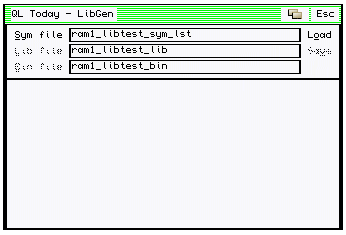
\includegraphics[width=0.65\textwidth]{Content/images/libgen_2.png}
\caption{How LibGen Currently Looks}
\label{fig:HowLibGenCurrentlyLooks}
\end{figure}

%Reference by See \figurename~\ref{fig@YourLabelHere}

We have now almost completed step 3. It is now time to complete step
    3 and move on to step 4. Change the code for the `Sym file' loose item's
    hit routine to the following.

\begin{lstlisting}[firstnumber=1,]
;---------------------------------------------------------------------
; SYM FILE loose item action routine.
;---------------------------------------------------------------------
afun0_2  movem.l d5-d7/a0-a4,-(a7) Preserve important registers.
         bsr.s li_unav           Make LI status unavailable.
         bsr sym_hit             Do it all.
         movem.l (a7)+,d5-d7/a0-a4 Restore important registers.
         cmpi.w #27,d1           Did we abort the edit?
         beq li_reset            Yes, bale out.
         bsr.s li_avail          Make LI status available, if all ok.
         bra li_reset            Make Sym file available.
\end{lstlisting}

The changes are quite simple. We call out to a subroutine -{}
 \texttt{li\_unav} -{} to change the status for all loose items
    from `Lib file' onwards to become unavailable. As we are potentially
    changing the symbol file name in this action routine, we cannot allow
    incorrect data to be used by the Library and Binary file names.

After returning from the main \texttt{sym\_hit} code, we
    check to see if the user aborted the edit with the ESC key. If so, then we
    know that the symbol file name currently on display is potentially
    garbage, and we exit leaving only the `Sym file' loose item
    available.

If the user successfully entered a symbol file name and did not
    abort the edit, we call the routine at \texttt{li\_avail} to
    set all the loose items, except `Save' to available. `Save' will be
    enabled by the actions of the `Load' loose item later.

\begin{lstlisting}[firstnumber=1,]
;---------------------------------------------------------------------
; Reset all Loose Items, affected by hitting "Sym file" to unavailable
; WSI_MKUN = $11 if you are wondering.
;---------------------------------------------------------------------
li_unav  move.b #wsi_mkun,ws_litem+li_libfile(a1)  Make Libfile unavailable
         move.w #$1111,ws_litem+li_load(a1)        Make Load and Save unavailabe
         move.b #wsi_mkun,ws_litem+li_binfile(a1)  Make Binfile unavailable
         bra.s li_rdrw

;---------------------------------------------------------------------
; Reset all Loose Items, affected by hitting "Sym file" to available
; except "Save". WSI_MKAV = $10 if you are wondering.
;---------------------------------------------------------------------
li_avail move.b #wsi_mkav,ws_litem+li_libfile(a1)  Make Libfile available
         move.b #wsi_mkav,ws_litem+li_load(a1)     Make Load available, Save stays Unavailable
         move.b #wsi_mkav,ws_litem+li_binfile(a1)  Make Binfile available

li_rdrw  moveq #-1,d3
         jmp wm_ldraw(a2) 
\end{lstlisting}

The above code is all that is required to enable and disable the
    affected loose items. It is quite simple to do this as there are only 4
    loose items affected and the status bytes for those four are consecutive
    in the status area. Also, for efficiency, we set all 4 as desired, and
    make one single call to \texttt{wm\_ldraw} rather than one call
    per loose item.

\begin{note}
You may remember that I mentioned, way back at the start, that
      there was more than one way to set the status bytes for these 4 loose
      items? Well, the code above is the other way. On a QPC or other device,
      running a 68000 or higher processor, I could have just used a MOVE.L
      \$11111111, WS\_LITEM+LI\_LIBFILE(A1) instruction as the make unavailable
      code. However, because li\_libfile is an odd number, that causes an
      address exception on the 68008 and 68010 processors. The standard QL has
      a 68008 of course.

The above code did in fact use the instruction mentioned. And it
      worked perfectly on my QPC which emulates a 68020, but, as noted in
 Section~\ref{ch33-errata}, this will fail miserably on a standard
      QL so this code is changed from that which first appeared in QL
      Today.
\end{note}

If you now assemble and run the application, HIT `Sym file' and type
    something in. If you abort the edit with ESC then the loose items remain
    disabled. If you press ENTER (or up/down arrows) then the loose items are
    enabled. `Save' remains disabled at all times.

\section{Handling the Lib File Loose Item}
\label{ch32-handling-lib-file}%\hyperlabel{ch32-handling-lib-file}%

There's not much happens when the user HITs the `Lib file' loose
    item. The user is allowed to change the default name, chosen for the
    library file, from that defaulted by LibGen.
    The defaults for this option and the binary file are based on the original
    symbol file which itself is based on the original source file name.

For example, if you assemble a source file named
 \nolinkurl{ram1_libtest_asm}, you will get a generated binary
    file of \nolinkurl{ram1_libtest_bin}, a listing of the code in
 \nolinkurl{ram1_libtest_lst} and a symbol file of
 \nolinkurl{ram1_libtest_sym}.

Using George's sym\_bin utility, you
    convert \nolinkurl{ram1_libtest_sym} into
 \nolinkurl{ram1_libtest_sym_lst}. It is this latter file that
 LibGen processes for you.

Based on the name of this latter file, LibGen chooses
 \nolinkurl{ram1_libtest_lib} for the library file -{} the one
    containing an `IN' and a `BIN' instruction, and for the actual binary file
    making up the library, chooses
 \nolinkurl{ram1_libtest_bin}.

In most cases, these defaults will be fine, but at least
 LibGen gives you the ability to change them as
    desired. After all, it's not wise to keep your various library files on
 \nolinkurl{ram1_} is it!

The code for the `Lib file' hit routine is as follows. This replaces
    the existing dummy code already in the main source file.

\begin{lstlisting}[firstnumber=1,]
;---------------------------------------------------------------------
; LIB FILE loose item action routine.
;---------------------------------------------------------------------
afun0_3  movem.l d5-d7/a0-a4,-(a7) Preserve important registers.
         bsr lib_hit             Do it all.
         movem.l (a7)+,d5-d7/a0-a4 Restore important registers.
         bra li_reset            Make Lib file available.
\end{lstlisting}

As before, I tend to prefer the actual hit routine to be small. The
    above code simply preserves the desired registers, calls out to the
 \texttt{lib\_hit} code, then restores the registers and exits
    resetting the `Lib file' loose item to available. You will see that it
    remains in a selected state until you complete the edit.

\begin{lstlisting}[firstnumber=1,]
;---------------------------------------------------------------------
; This code carries out all the nasty work for a hit on the Lib file
; loose item. It is called from afun0_3 above.
;---------------------------------------------------------------------
lib_hit  moveq #iw_libfile,d1    Info window number in d1.w.
         lea lib_buffer,a3       Current lib file buffer.
         moveq #1,d2             Blue Ink when editing.
         bsr iw_input            Get input from desired info window.
         bmi.s lf_exit           Something went wrong, bale out.
\end{lstlisting}

Nothing much of interest here, the processing is almost identical to
    that we have seen already for allowing the user the ability to type a
    symbol file name. We don't have to check for the ESC key terminating the
    edit because we always, unless there was an error, exit via the tidy up
    code at \texttt{lf\_ok}. Remember that our library routine
 \texttt{iw\_input} copies the data from the working edit buffer
    back to the correct location on a successful edit.

\begin{lstlisting}[firstnumber=1,]
;---------------------------------------------------------------------
; Print the lib file name. We do this at the end of a normal edit and
; when the user aborts with ESC. This keeps the info window tidy.
;---------------------------------------------------------------------
lf_ok    moveq #iw_libfile,d1    Information window desired.
         moveq #0,d2             Black ink.
         lea lib_buffer,a3       Filename to print.
         bsr iw_print            Print it.
         
lf_exit rts 
\end{lstlisting}

The code above, you may notice, doesn't preserve the terminating
    character in D1. There isn't really any requirement to do so in the
    handling of a `Lib file' HIT.

\section{Handling the Bin File Loose Item}
\label{ch32-handling-bin-file}%\hyperlabel{ch32-handling-bin-file}%

The code for handling a hit on the `Bin file' loose item is almost
    identical to the above. It will be shown here without further
    discussion.

\begin{lstlisting}[firstnumber=1,]
;---------------------------------------------------------------------
; BIN FILE loose item action routine.
;---------------------------------------------------------------------
afun0_6  movem.l d5-d7/a0-a4,-(a7) Preserve important registers.
         bsr bin_hit             Do it all.
         movem.l (a7)+,d5-d7/a0-a4 Restore important registers.
         bra li_reset            Make Bin file available.

;---------------------------------------------------------------------
; This code carries out all the nasty work for a hit on the Bin file
; loose item. It is called from afun0_6 above.
;---------------------------------------------------------------------
bin_hit  moveq #iw_binfile,d1    Info window number in d1.w.
         lea bin_buffer,a3       Current bin file buffer.
         moveq #1,d2             Blue ink when editing.
         bsr iw_input            Get input from desired info window.
         bmi.s bf_exit           Something went wrong, bale out.

;---------------------------------------------------------------------
; Print the bin file name. We do this at the end of a normal edit and
; when the user aborts with ESC. This keeps the info window tidy.
;---------------------------------------------------------------------
bf_ok    moveq #iw_binfile,d1    Information window desired.
         moveq #0,d2             Black ink.
         lea bin_buffer,a3       Filename to print.
         bsr iw_print            Print it.
         
bf_exit rts 
\end{lstlisting}

If you assemble the code and execute it you should find that
    everything works as desired.

\section{Coming Up...}
\label{ch32-the-end}%\hyperlabel{ch32-the-end}%

In the next chapter we will add the real meat of
    the utility -{} the ability to load a file, select which entries you want
    from a menu, and then save those entries out to a file suitable for
    inclusion in future assembly programs.
